\section{Deep Generative Models}
\frame{\tableofcontents[currentsection]}


\begin{frame}{Generative Model with NN Likelihood}
\begin{block}{Goal}
Define model $ p(x,z|\theta) = p(x|z,\theta)p(z) $ where the likelihood $ p(x|z,\theta) $ is given by a neural
network. 

~

We fix $ p(z) $ for simplicity.
\end{block}

\end{frame}

\begin{frame}{Example: Language Model}

	A deterministic language model is {\bf one} distribution over observations:
	\begin{equation*}
		p(x|\theta) = \prod_{i=1}^n p(x_i|x_{<i}, \theta)
	\end{equation*}
	
	Every sentence gets mapped from the same conditioning context, namely, the beginning of sequence symbol.


\end{frame}

\begin{frame}{Example: Language Model (cont.)}
	
	With latent variables we can model the data as a draw from a complex marginal, which mixes conditionals from different points in space
	\begin{equation*}
		p(x|\theta) = \int p(\textcolor{blue}{z}) \prod_{i=1}^n p(x_i|\textcolor{blue}{z}, x_{<i}, \theta) \dd \textcolor{blue}{z}
	\end{equation*}
	
	~ \pause
	
	Good training can lead to considerable amount of structure in the posterior
	\begin{equation*}
		p(z|x, \theta) = \frac{p(z)p(x|z, \theta)}{\alert{p(x|\theta)}}
	\end{equation*}

\end{frame}

\begin{frame}[plain]%{Example: Language Model (illustration)}

	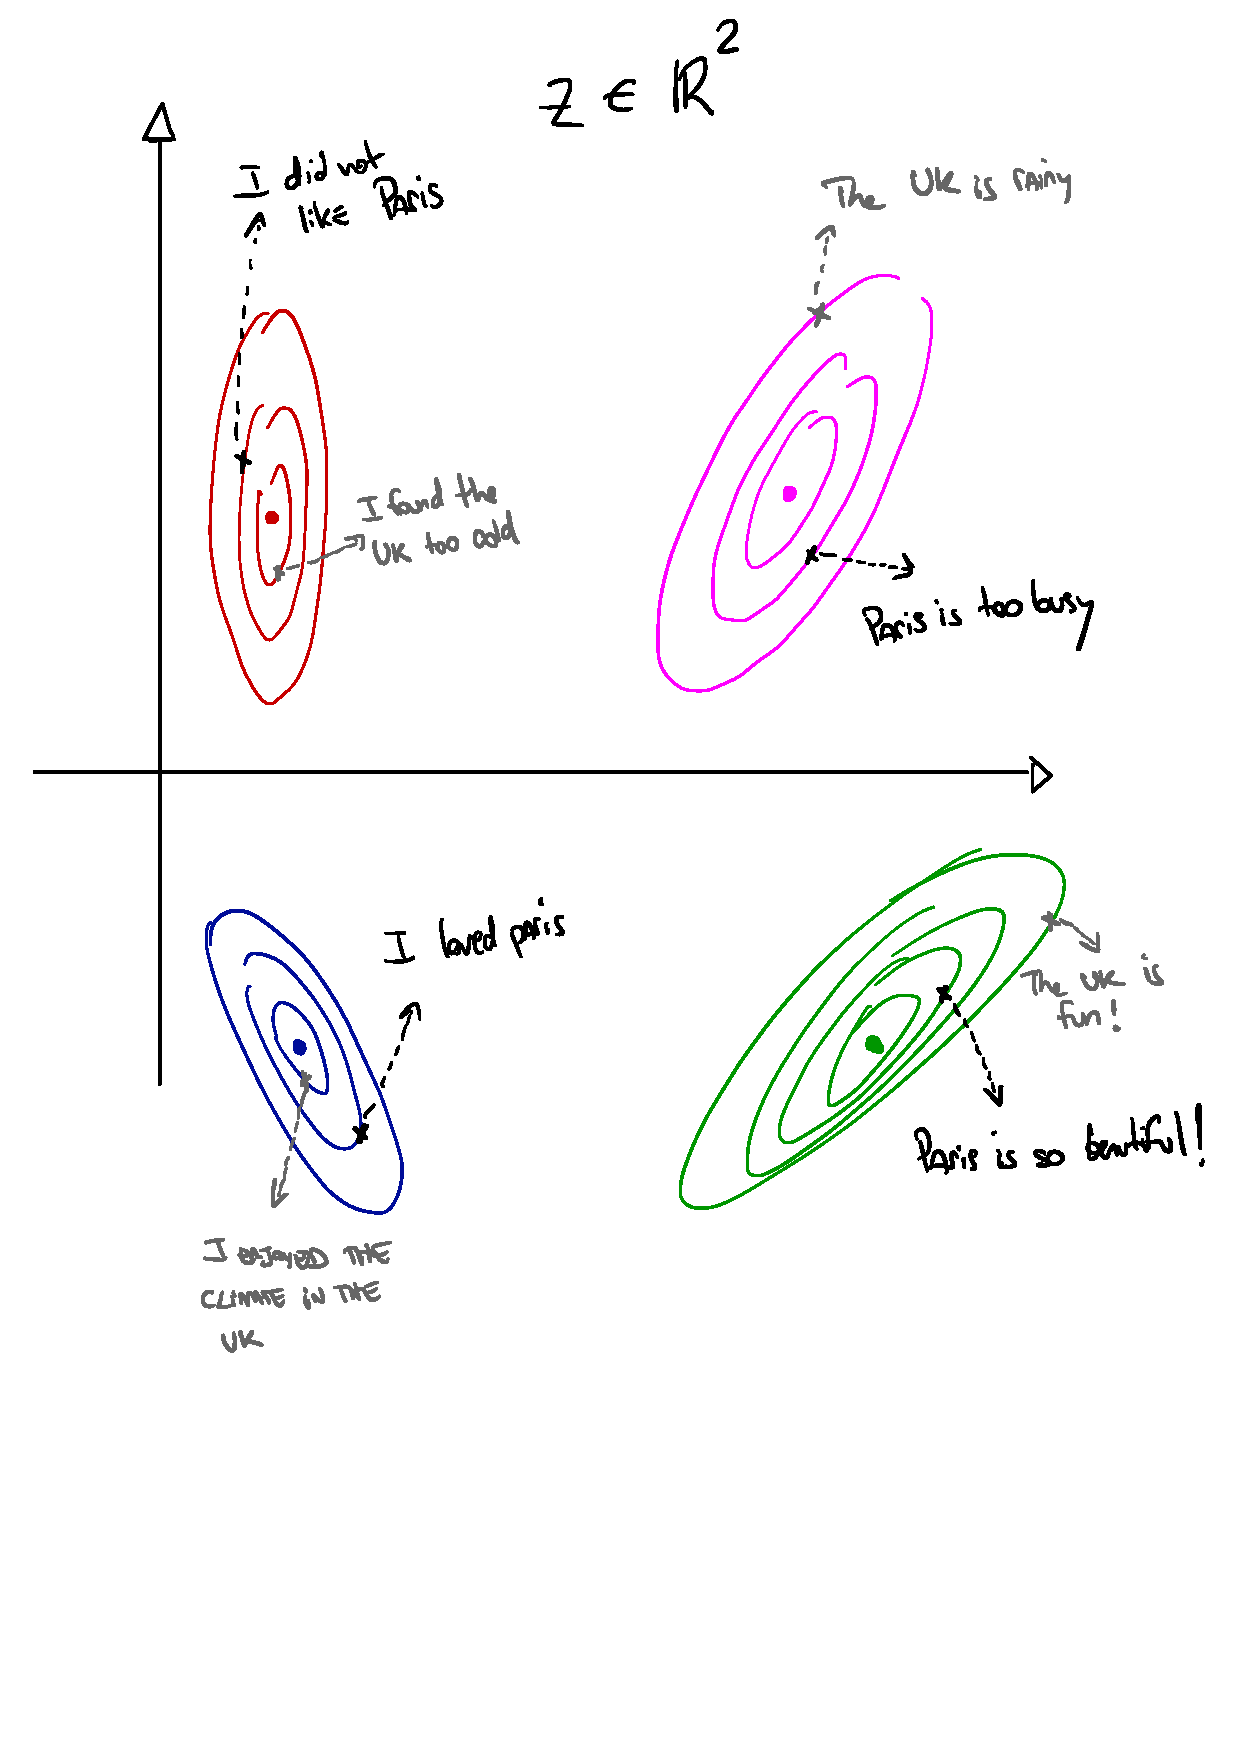
\includegraphics[scale=0.4]{VAE-example}

\end{frame}

\begin{frame}{Example: Language Model (architecture)}

Generative model:
\begin{equation*}
\begin{aligned}
Z & \sim \mathcal N(0, I) \\
X_i|z, x_{<i} & \sim \Cat(f(z, x_{<i}; \theta))
\end{aligned}
\end{equation*}

\pause 
Example architecture:
\begin{equation*}
\begin{aligned}
h_0 &= \tanh(W^{(\text{init})} z + b^{(\text{init})}) \\ \pause
h_i &= \rnn(h_{i-1}, E_{x_{i-1}}; \theta_{\text{rnn}}) \\ \pause
f(z, x_{<i}) &= \softmax(W^{(\text{out})} h_i + b^{(\text{out})}) \\ \pause
\theta &= \theta_{\text{rnn}} \cup \{W^{(\text{init})}, b^{(\text{init})}, W^{(\text{out})}, b^{(\text{out})}\}
\end{aligned}
\end{equation*}


\end{frame}

\begin{frame}{Generative Model with NN Likelihood}
\begin{block}{Goal}
Define model $ p(x,z|\theta) = p(x|z,\theta)p(z) $ where the likelihood $ p(x|z,\theta) $ is given by a neural
network. (We fix $ p(z) $ for simplicity.)
\end{block}

\begin{block}{Problem}
$ p(x|\theta) = \int p(z) p(x|z,\theta)  \dd z $ is intractable!
\end{block}
\end{frame}



\section{Variational Autoencoders}
\frame{\tableofcontents[currentsection]}

\begin{frame}{Solution: Variational Inference}

\vspace{-10pt}
\begin{small}
\begin{equation*}
\begin{aligned}
\log p(x|\theta) &\geq \overbrace{\E[q(z|x, \lambda)]{\log p(x,z|\theta)} + \Ent{q(z|x, \lambda)}}^{\ELBO} \\ 
\pause
&= \E[q(z|x, \lambda)]{\log p(x|z, \theta) + \log p(z)} + \Ent{q(z|x, \lambda)} \\ \pause
&= \E[q(z|x, \lambda)]{\log p(x|z, \theta)} - \KL{q(z|x, \lambda)}{p(z)}
\end{aligned}
\end{equation*}
\end{small}

\pause

\vspace{-20pt}
\begin{equation*}
\argmax_{\theta,\lambda} ~ \E[q(z|x, \lambda)]{\log p(x|z, \theta)} - \KL{q(z|x, \lambda)}{p(z)}
\end{equation*}


\pause

\begin{itemize}
	\item assume $\KL{q(z|x, \lambda)}{p(z)}$  analytical\\
	true for exponential families \pause
	\item approximate $\E[q(z|x, \lambda)]{\log p(x|z, \theta)}$ by sampling\\
	feasible because  $q(z|x, \lambda)$ is simple
\end{itemize}


\end{frame}

\begin{frame}{Generator Network Gradient}
\vspace{-10pt}
\begin{equation*}
\begin{aligned}
&\pdv{\theta}\E[q(z|x,\lambda)]{\log p(x|z,\theta)} - \overbrace{\KL{q(z|x,\lambda)}{p(z)}}^{constant} \\ \pause 
&=\E[q(z|x,\lambda)]{\pdv{\theta}\log p(x|z,\theta)} \\ \pause
&\overset{\text{MC}}{\approx} \frac{1}{S}\sum_{i=1}^{S}
\pdv{\theta} \log p(x|z_{i},\theta) \\
&\textcolor{gray}{\text{where }z_i \sim q(z|x, \lambda)}
\end{aligned}
\end{equation*}
\pause
\center{Note: $ q(z|x,\lambda) $ does not depend on $ \theta $.}
\end{frame}

\begin{frame}{Inference Network Gradient}
\begin{equation*}
\begin{aligned}
&\pdv{\lambda}\left[\E[q(z|x,\lambda)]{\log p(x|z,\theta)} - \KL{q(z|x,\lambda)}{p(z)} \right] \\ \pause
=&\pdv{\lambda}\E[q(z|x,\lambda)]{\log p(x|z,\theta)} - \underbrace{\pdv{\lambda}\KL{q(z|x,\lambda)}{p(z)}}_{\text{analytical computation}} \\
\end{aligned}
\end{equation*}
\pause
\center{The first term again requires approximation by sampling}
\end{frame}

\begin{frame}{Inference Network Gradient}


\begin{equation*}
\begin{aligned}
&\pdv{\lambda}\E[q(z|x,\lambda)]{\log p(x|z,\theta)} \\ \pause
&= \pdv{\lambda} \intl{q(z|x,\lambda)\log p(x|z,\theta)}{z} \\ \pause
&= \intl{\alert{\pdv{\lambda} q(z|x,\lambda)}\log p(x|z,\theta)}{z}
\end{aligned}
\end{equation*}
\pause
Not an expected gradient!
\end{frame}

\begin{frame}{Score function estimator?}

	Can we apply the log-derivative trick? 
	\vspace{-10pt}
	
	\begin{equation*}
	\begin{aligned}
	&\pdv{\lambda}\E[q(z|x,\lambda)]{\log p(x|z,\theta)} \\
	&= \int \alert{\pdv{\lambda} q(z|x,\lambda)}\log p(x|z,\theta) \dd z \\ \pause
	&= \int \textcolor{blue}{q(z|x,\lambda) \pdv{\lambda} \log q(z|x,\lambda)}\log p(x|z,\theta) \dd z \\ \pause
	&= \mathbb E_{q(z|x,\lambda)}\left[ \log p(x|z,\theta) \pdv{\lambda} \log q(z|x,\lambda)  \right]
	\end{aligned}
	\end{equation*}
	
	Yes, it's a general result!

\end{frame}

\begin{frame}{What about variance?}

	The learning signal can only scale the gradient:
	\begin{equation*}
	\begin{aligned}
	&\pdv{\lambda}\E[q(z|x,\lambda)]{\log p(x|z,\theta)} \\
	&= \mathbb E_{q(z|x,\lambda)}\left[ \alert{\log p(x|z,\theta)} \pdv{\lambda} \log q(z|x,\lambda)  \right]
	\end{aligned}
	\end{equation*}
	
	\pause
	
	Can we do better? 
	
\end{frame}
\begin{frame}{Inference Network Gradient}
\begin{block}{Problem}
We need to re-express the gradient, but the measure of integration depends on $\lambda$
	\begin{equation*}
	\begin{aligned}
	&\pdv{\alert{\lambda}}\E[q(z|x,\alert{\lambda})]{\log p(x|z,\theta)}
	\end{aligned}
	\end{equation*}
	
	\pause
	
	What if we could re-express $q(z|x, \lambda)$ in terms of some other distribution that does not depend on $\lambda$?

\end{block}
\end{frame}


\begin{frame}{Inference Network Gradient}
\begin{block}{Reparametrisation trick}
Find a transformation $ h: z \mapsto \epsilon $ such that $ \epsilon $ does not depend on $ \lambda $.
\begin{itemize}
\item $ h(z, \lambda) $ needs to be invertible
\item $ h(z, \lambda) $ needs to be differentiable
\pause
\item $ h(z, \lambda) = \epsilon $
\item $ h^{-1}(\epsilon, \lambda) = z $ 
\end{itemize}
\end{block}
\end{frame}

\begin{frame}{Gaussian Transformation}

\textbf{Affine property}
\begin{equation*}
Az + b \sim \NDist{\mu + b}{A\Sigma A^{T}} \text{ for } z \sim \NDist{\mu}{\Sigma}
\end{equation*}
\pause
\textbf{Special case}
\begin{equation*}
Az + b \sim \NDist{b}{A A^{T}} \text{ for } z \sim \NDist{0}{\IMatrix}
\end{equation*}

\end{frame}

\begin{frame}{Gaussian Transformation}

Let an inference network compute
\begin{equation*}
\begin{aligned}
u &= \mu(x;\lambda) & & s&= \sigma(x;\lambda)
\end{aligned}
\end{equation*}
for a posterior $Z \sim \mathcal N(u, s^2)$, then we have: \pause
\begin{equation*}
h(z, \lambda; x) = \frac{z - \mu(x;\lambda)}{ \sigma(x; \lambda) } = \epsilon \sim \NDist{0}{\IMatrix} 
\end{equation*} \pause
and conversely, for $\epsilon \sim \mathcal N(0, I)$, we have:
\begin{equation*}
h^{-1}(\epsilon, \lambda; x) = \mu(x;\lambda) + \sigma(x; \lambda) \odot \epsilon = z  \sim \mathcal N(u, s^2)
\end{equation*}

\end{frame}

\begin{frame}{Inference Network Gradient}

\begin{equation*}
\begin{aligned}
&= \pdv{\lambda} \intl{q(z|x,\lambda)\log p(x|z,\theta)}{z} \\ \pause
&= \pdv{\lambda} \intl{\alert{q(\epsilon)} \loga{ p(x | \alert{\overbrace{h^{-1}(\epsilon, \lambda)}^{=z}},\theta)}}{\alert{\epsilon}} \\ \pause
&= \intl{q(\epsilon) \pdv{\lambda} \left[ \log p(x| \overbrace{h^{-1}(\epsilon, \lambda)}^{=z}, \theta)\right] }{\epsilon}
\end{aligned}
\end{equation*}
\end{frame}

\begin{frame}{Inference Network Gradient}
\vspace{-10pt}
\begin{equation*}
\begin{aligned}
&\E[q(\epsilon)]{\pdv{\lambda} \log p(x| \overbrace{h^{-1}(\epsilon, \lambda)}^{=z}, \theta)} \\ \pause
\overset{\text{MC}}{\approx} &\frac{1}{S}\sum_{i=1}^{S} \pdv{\lambda} \log p(x| \overbrace{h^{-1}(\epsilon_i, \lambda)}^{=z}, \theta) \\
&\textcolor{gray}{\text{where }\epsilon_i \sim q(\epsilon)} \\ \pause
\overset{\text{MC}}{\approx} &\frac{1}{S}\sum_{i=1}^{S} \underbrace{\pdv{z} \log p(x| \overbrace{h^{-1}(\epsilon_i, \lambda)}^{=z}, \theta) \times \pdv{\lambda} h^{-1}(\epsilon_i, \lambda)}_{\text{chain rule}}
%= &\E[q(\epsilon)]{\frac{d}{dz} \log p(x| \overbrace{h^{-1}(\epsilon, \lambda)}^{=z}, \theta)\times \frac{d}{d\lambda} h^{-1}(\epsilon, \lambda)}\\ \pause
%\overset{\text{MC}}{\approx} &\frac{1}{S}\sum_{i=1}^{S} \frac{d}{dz} \log p(x| \overbrace{h^{-1}(\epsilon, \lambda)}^{=z}, \theta) \times \frac{d}{d\lambda} h^{-1}(\epsilon, \lambda)
\end{aligned}
\end{equation*}
\end{frame}

\begin{frame}{Derivatives of Gaussian transformation}
Recall: $$\quad h^{-1}(\epsilon, \lambda) = \mu(x,\lambda) + \sigma(x,\lambda) \odot \epsilon \ . $$

We get two gradient paths! \pause \\

\begin{itemize}
	\item one is \alert{deterministic}\\
	$\pdv{h^{-1}(\epsilon, \lambda)}{\mu(x,\lambda)} = \pdv{\mu(x,\lambda)}[\mu(x,\lambda) + \sigma(x,\lambda) \odot \epsilon] = 1$ \pause
	\item the other is  \alert{stochastic}\\
	$\pdv{h^{-1}(\epsilon, \lambda)}{\sigma(x,\lambda)} = \pdv{\sigma(x,\lambda)}[ \mu(x,\lambda) + \sigma(x,\lambda) \odot \epsilon] = \epsilon$
\end{itemize}

\end{frame}

\begin{frame}{Gaussian KL}
\begin{block}{ELBO}
\begin{equation*}
\E[q(z|x,\lambda)]{\log p(x|z,\theta)} - \KL{q(z|x,\lambda)}{p(z)}
\end{equation*}
\end{block}
\pause
Analytical computation of $ -\KL{q(z|x,\lambda)}{p(z)} $:
\begin{equation*}
\frac{1}{2}\sum_{i=1}^{N}\left(1 + \loga{\sigma^{2}_{i}} -
\mu^{2}_{i} - \sigma^{2}_{i} \right)
\end{equation*}
\end{frame}

\begin{frame}{Computation Graph}
\begin{figure}
\begin{tikzpicture}[node distance=1cm]
\node[rectangle, draw, rounded corners, thick] (input) {$x$};
\node[rectangle, draw, rounded corners, thick, above left=of input] (mu) {$ \mu $};
\node[rectangle, draw, rounded corners, thick, above right=of input] (var) {$ \sigma $};
\node[rectangle, draw, rounded corners, thick, above right= of mu] (z) {$ z $};
\node[rectangle, fill=blue!20, thick, above of= z, rounded corners, draw, node distance=1.5cm] (output) {$ x $};

\draw[->, thick] (input) -- (mu) node[midway, above, rotate=315] {$ \lambda $};
\draw[->, thick] (input) -- (var) node[midway, above, rotate=45] {$ \lambda $};
\draw[->, thick] (mu) edge (z);
\draw[->, thick] (var) edge (z);
\draw[->, thick] (z) -- (output) node[midway, right] {$ \theta $};

\pause
\node[draw=orange, thick, rectangle, fit= (input) (mu) (var), rounded corners] {};
\node[left= of mu] (inference) {\textcolor{orange}{inference model}};

\pause
\node[draw=blue!50, thick, rectangle, fit= (z) (output), rounded corners] {};
\node[above= of inference] (generation) {\textcolor{blue!50}{generation model}};

\pause
\node[circle, draw, thick ,right =of var, xshift=-.5cm] (epsilon) {$ \epsilon $};
\node[right = of epsilon, xshift=-1cm] (stdNormal) {$ \sim \NDist{0}{1} $};
\draw[->, thick] (epsilon) edge (var);

\pause
\node[above= of mu, rectangle, fill=blue!20, thick, rounded corners, draw,] (KLmu) {$ \KullbackLeibler $};
\draw[->, thick] (mu) edge (KLmu);
\node[above= of var, rectangle, fill=blue!20, thick, rounded corners, draw,] (KLvar) {$ \KullbackLeibler $};
\draw[->, thick] (var) edge (KLvar);
\end{tikzpicture}
\end{figure}
\end{frame}


\begin{frame}{Example: Unigram Document Model}


\begin{columns}
	\begin{column}{0.2\textwidth}
	\begin{tikzpicture}
    % Define nodes
    \node[latent]		(z)		{$ z $};
    \node[obs, below = of z]		(x)		{$ x $};
    \node[right = of x]		(theta)		{$ \theta $};
    
    % Connect nodes
    \edge{z,theta}{x};
    
    % add plates
    \plate {x-sentence} {(x)} {$ n $};
   
    %\node[right = of z]		(lambda)		{$ \lambda $};   
    %\edge[dashed, bend right]{x}{z};
    %\edge{lambda}{z};
    \end{tikzpicture}
    \end{column}
    \begin{column}{0.75\textwidth}
    	Generative story 
    	\begin{itemize}
			\item Draw a document embedding $Z \sim \mathcal N(0, I)$
			\item Draw $n$ words\\
			$X_i|z \sim \Cat(f(z; \theta))$
		\end{itemize}
    \end{column}
    \end{columns}
    \pause
    
    ~
    
    Designing $f(z, \theta)$    \pause
    \begin{equation*}
	\begin{aligned}						
		h &= \tanh(W_1z+b_1) \\ \pause
		f(z, \theta) &= \alert{\softmax}(W_2h + b_2) \\		\pause
		\theta &= \{W_1, b_1, W_2, b_2\}
	\end{aligned}
	\end{equation*}
	

\end{frame}

\begin{frame}{Example: Unigram Document Model}


\begin{columns}
	\begin{column}{0.2\textwidth}
	\begin{tikzpicture}
    % Define nodes
    \node[latent]		(z)		{$ z $};
    \node[obs, below = of z]		(x)		{$ x $};
    \node[right = of x]		(theta)		{$ \theta $};
    
    % Connect nodes
    \edge{z,theta}{x};
    
    % add plates
    \plate {x-sentence} {(x)} {$ n $};
   
    %\node[right = of z]		(lambda)		{$ \lambda $};   
    %\edge[dashed, bend right]{x}{z};
    %\edge{lambda}{z};
    \end{tikzpicture}
    \end{column}
    \begin{column}{0.75\textwidth}
    	Generative story 
    	\begin{itemize}
			\item Draw a document embedding $Z \sim \mathcal N(0, I)$
			\item Draw $n$ words\\
			$X_i|z \sim \Cat(f(z; \theta))$
		\end{itemize}
    \end{column}
    \end{columns}
    
    
    ~
    
	Likelihood \pause
	\begin{small}
    \begin{equation*}
	\begin{aligned}						
		p(x|z, \theta) &= \prod_{i=1}^n p(x_i|z, \theta) \pause = \prod_{i=1}^n \Cat(x_i|\underbrace{f(z; \theta)}_{=\psi}) \\ \pause
		&= \prod_{i=1}^n \psi_{x_i}
	\end{aligned}
	\end{equation*}
	\end{small}

\end{frame}


\begin{frame}{Example: Unigram Document Model}


\begin{columns}
	\begin{column}{0.2\textwidth}
	\begin{tikzpicture}
    % Define nodes
    \node[latent]		(z)		{$ z $};
    \node[obs, below = of z]		(x)		{$ x $};
    \node[right = of x]		(theta)		{$ \theta $};
    
    % Connect nodes
    \edge{z,theta}{x};
    
    % add plates
    \plate {x-sentence} {(x)} {$ n $};
   
    %\node[right = of z]		(lambda)		{$ \lambda $};   
    %\edge[dashed, bend right]{x}{z};
    %\edge{lambda}{z};
    \end{tikzpicture}
    \end{column}
    \begin{column}{0.75\textwidth}
    	Generative story 
    	\begin{itemize}
			\item Draw a document embedding $Z \sim \mathcal N(0, I)$
			\item Draw $n$ words\\
			$X_i|z \sim \Cat(f(z; \theta))$
		\end{itemize}
    \end{column}
    \end{columns}
    
    
    ~
    
	Marginal \pause
	\begin{small}
    \begin{equation*}
	\begin{aligned}						
		p(x|\theta) &= \int p(z) \prod_{i=1}^n p(x_i|z, \theta) \dd{z} \pause \\
		&= \alert{\int \mathcal N(z|0, I)} \prod_{i=1}^n \Cat(x_i|\alert{f(z; \theta)}) \alert{\dd{z}}
	\end{aligned}
	\end{equation*}
	\end{small}

\end{frame}

\begin{frame}{Example: Unigram Document Model}


\begin{columns}
	\begin{column}{0.75\textwidth}  
   		\textcolor{blue}{Inference model}
		\begin{itemize}
			\item $Z|x \sim \mathcal N(\mu(x; \lambda), \sigma(x; \lambda)^2)$
		\end{itemize}
    \end{column}
	\begin{column}{0.2\textwidth}
	\begin{tikzpicture}
    % Define nodes
    \node[latent]		(z)		{$ z $};
    \node[obs, below = of z]		(x)		{$ x $};
    \node[right = of x]		(theta)		{$ \theta $};
    
    % Connect nodes
    \edge{z,theta}{x};
    
    % add plates
    \plate {x-sentence} {(x)} {$ n $};
   
    \node[right = of z]		(lambda)		{$ \lambda $};   
    \edge[dashed, blue, bend right]{x}{z};
    \edge[blue]{lambda}{z};
    \end{tikzpicture}
    \end{column}    
    \end{columns}
    \pause
    
    Designing the \emph{inference network}\pause
    \vspace{-10pt}
    \begin{columns}
    \begin{column}{0.35\textwidth}
    \begin{equation*}
	\begin{aligned}		
		s &= \sum_{i=1}^n E_{x_i} \pause \\
		h &= \tanh(M_1s+c_1)  \pause 		
	\end{aligned}
	\end{equation*}
	\end{column}
	\begin{column}{0.6\textwidth}
	\begin{equation*}
	\begin{aligned}		
		\mu(x; \lambda) &= M_2h + c_2  \pause \\
		\sigma(x; \lambda) &= \alert{\softplus}(M_3h + c_3)  \pause \\
		\lambda &= \{E, M_1^3, c_1^3\}
	\end{aligned}
	\end{equation*}
	\end{column}
	\end{columns}
	

\end{frame}


\begin{frame}{Example: Unigram Document Model}

\begin{columns}
	\begin{column}{0.75\textwidth}  

		Generative Model
		\begin{itemize}
			\item Prior: $Z \sim \mathcal N(0, I)$
			\item Likelihood: $X_i|z \sim \Cat(f(z; \theta))$
		\end{itemize}
   		Inference Model
		\begin{itemize}
			\item $Z|x \sim \mathcal N(\mu(x; \lambda), \sigma(x; \lambda)^2)$
		\end{itemize}
    \end{column}
	\begin{column}{0.2\textwidth}
	\begin{tikzpicture}
    % Define nodes
    \node[latent]		(z)		{$ z $};
    \node[obs, below = of z]		(x)		{$ x $};
    \node[right = of x]		(theta)		{$ \theta $};
    
    % Connect nodes
    \edge{z,theta}{x};
    
    % add plates
    \plate {x-sentence} {(x)} {$ n $};
   
    \node[right = of z]		(lambda)		{$ \lambda $};   
    \edge[dashed, blue, bend right]{x}{z};
    \edge[blue]{lambda}{z};
    \end{tikzpicture}
    \end{column}    
    \end{columns}
    \pause
    
    \vspace{10pt}
    
    \alert{ELBO}
    \vspace{-10pt}
	\begin{equation*}
	\begin{aligned}		
		\log p(x|\theta) &\ge \mathbb E_{\epsilon \sim \mathcal N(0, I)}\left[ \textstyle\sum_{i=1}^n \log \psi_{x_i}\right] \\
		&- \KL{\mathcal N(u, s^2)}{\mathcal N(0, I)}
	\end{aligned}
	\end{equation*}
	\textcolor{gray}{{\small where $u = \mu(x; \lambda)$, $s = \sigma(x; \lambda)$, and $\psi = f(z = u + \epsilon \odot s, \theta)$ }}

\end{frame}

\section{Posterior collapse}

\begin{frame}{Posterior collapse}
We are point estimating $p(x,z|\theta)$ along with $q(z|x, \lambda)$
\begin{itemize}
	\item where $p(x,z|\theta) = p(z) \prod_{i=1}^n p(\textcolor{blue}{x_i}|\alert{z}, \textcolor{blue}{x_{<i}}, \theta)$ \pause
	\item if we pick $\theta$ such that $\textcolor{blue}{X_i} \perp \alert{Z} \mid \textcolor{blue}{X_{<i}}$, then  \pause
	\begin{equation*}
	\begin{aligned}
		p(z|x, \theta) &=  \frac{p(z) \prod_{i=1}^n p(\textcolor{blue}{x_i}|\alert{z}, \textcolor{blue}{x_{<i}}, \theta) }{p(x|\theta)}  \\ \pause
		&= \frac{p(z) \prod_{i=1}^n p(\textcolor{blue}{x_i}|\textcolor{blue}{x_{<i}}, \theta) }{p(x|\theta)}  \pause = \frac{p(z)p(x|\theta)}{p(x|\theta)} \\ \pause
		&= p(z) \pause
	\end{aligned}	
	\end{equation*}
	\item the {\bf true posterior} \emph{collapses} to the prior 
	\end{itemize}
\end{frame}

\begin{frame}{Strong generators}

If your likelihood model is able to express dependencies between the output variables (e.g. an RNN), the model may simply ignore the latent code.

~

Note that though $X \perp Z$ (or $X_i \perp Z \mid X_{<i}$)\\
~ $\prod_{i=1}^n p(\textcolor{blue}{x_i}|\textcolor{blue}{x_{<i}}, \theta)$ \emph{still is} an exact factorisation of $p(x|\theta)$.

~

We call such models \emph{strong generators}.

\end{frame}

\begin{frame}{Diagnosing posterior collapse}

Fact: the \emph{rate} $R = \mathbb E_X[\KL{q(z|x, \lambda)}{p(z)}]$ is an upperbound on $I(X; Z|\lambda)$ \ack{$I(X;Z|\lambda) = \int \int q(x,z|\lambda) \log \frac{q(x,z|\lambda)}{q_\star(x)q(z|\lambda)} \dd x \dd z$ and $q(x,z|\lambda) = q_\star(x)q(z|x, \lambda)$.} \pause

\begin{itemize}
	\item if $\KL{q(z|x, \lambda)}{p(z)}$ is close to $0$ to most training instances, then $I(X; Z|\lambda)$ is $0$ or negligible; \pause
	\item greedy decoding $\argmax_{x_i} \log p(x_i|z, x_{<i})$ from a prior sample $z \sim p(z)$ is deterministic; \pause
	\item this does not mean ancestral samples from $p(x|z, \theta)$ will be bad
\end{itemize}


\end{frame}

\begin{frame}{KL scaling}


Gradually incorporate the KL term into the objective
\begin{equation*}
\E[q(z|x,\lambda)]{\log p(x|z,\theta)} - \beta \KL{q(z|x,\lambda)}{p(z)}
\end{equation*}
where $\beta$ starts at $0$ and goes to $1$ after a number of steps.

~ \pause

This sometimes helps reach better local optimum, but there are not guarantees. In fact, oftentimes, soon after we reach $1$, the posterior collapses again.
\end{frame}

\begin{frame}{Free bits}

Another strategy is to promote the posterior to deviate a bit from the prior by not penalising for the first few nats of information:
\begin{equation*}
\E[q(z|x,\lambda)]{\log p(x|z,\theta)} - \max(r, \KL{q(z|x,\lambda)}{p(z)})
\end{equation*}
where $r \ge 0$ is known as ``free bits''  

~

This is an attempt to promote solutions where $R \ge r$

\end{frame}

\begin{frame}{Attention!}

But note that if we scale down the KL term permanently, or allow too many free bits, then the conditional $p(x|z, \theta)$ will over-specialise to samples from the approximate posterior $q(z|x, \lambda)$. 
This can lead to bad generalisation and/or poor samples when generating from the prior.

\end{frame}

\begin{frame}{Variational Autoencoder}
\textbf{Advantages}
\begin{itemize}
\item Backprop training
\item Easy to implement
\item Posterior inference possible
\item One objective for both NNs
\item Amortised inference
\end{itemize}
\pause
\textbf{Drawbacks}
\begin{itemize}
\item Discrete latent variables are not possible
\item Optimisation may be difficult with several latent variables
\end{itemize}
\end{frame}

\begin{frame}{Summary}
\begin{itemize}
%\item When $ |\mathcal{X}| $ and $ |\mathcal{Z}| $ are not too large, we can do EM with features
%\item Otherwise use VI with simple approximation
\item Wake-Sleep: train inference and generation networks with separate objectives
\item VAE: train both networks with same objective
\item Reparametrisation
\begin{itemize}
\item  Transform parameter-free variable $ \epsilon $ into latent value $ z $
\item Update parameters with stochastic gradient estimates
\end{itemize}
\item If you employ strong generators, watch out for posterior collapse 
\end{itemize}
\end{frame}

\begin{frame}{Implementation}

Try one of our notebooks, e.g.
\begin{itemize}
	\item Original VAE: MNIST\\
	\url{https://github.com/vitutorial/VITutorial/blob/master/code/vae_notebook_pytorch.ipynb}
	\item SentenceVAE\\
	\url{https://github.com/probabll/dgm4nlp/tree/master/notebooks/sentencevae}	
	\item WordVAE \\
	\url{https://github.com/vitutorial/exercises/tree/master/WordVAE}
\end{itemize}
\end{frame}

\begin{frame}[allowframebreaks]{Literature}
\nocite{KingmaWelling:2013}
\nocite{HintonEtAl:1995}
\nocite{RezendeEtAl:2014}
\nocite{TitsiasLazarogredilla:2014}
%\nocite{BergkirkpatrickEtAl:2010}
\nocite{KucukelbirEtAl:2017}
\nocite{alemi2018fixing}
\nocite{chen2016variational}
\nocite{pelsmaeker2019effective}

\bibliographystyle{plainnat}
\bibliography{../../VI}
\end{frame}
